\subsection{Proposed Timeline}
%\todo[inline]{A Gantt chart, perhaps with critical tasks highlighted, to be detailed below}
Figure \ref{fig::gantt_chart} shows my proposed timeline to complete my thesis work. Most work is to be completed during the first semester of next year, though I have organised to get as much research complete over the summer break so I can use my time more appropriately during semester. The red bars show an alternate pathway to a working solution, if the \gls{pcie} digitizer or MATLAB is unable to perform the required task.
\begin{figure}[htbp!]
	\centering
	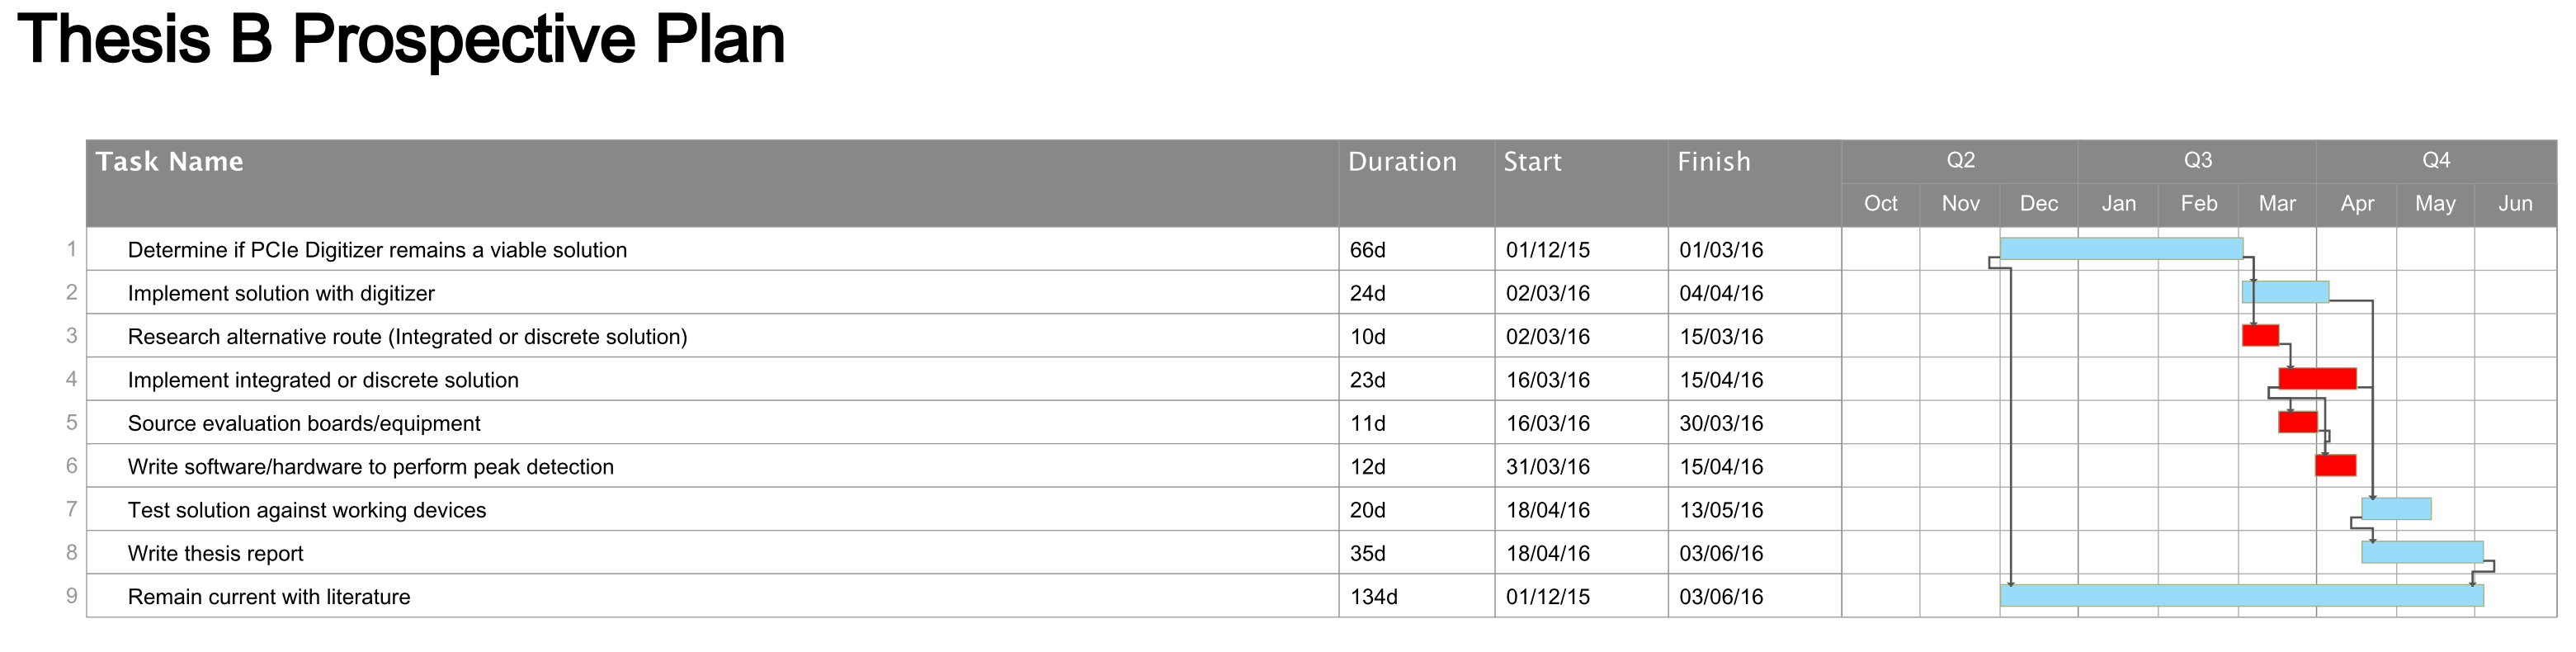
\includegraphics[width=\textwidth, height=0.3\textheight]{gantt_chart}
	\caption{Gantt Chart for Thesis B, beginning December}
	\label{fig::gantt_chart}
\end{figure}

\subsection{Description of Work}

The following lists are the final avenues available in utilizing the \gls{pcie} digitizer and MATLAB solution.
\begin{itemize}
	\item Software Triggering
	\item Continuous \gls{dma}
	\item Manual external triggering
\end{itemize}
By the beginning of semester I will be able to confirm or deny if any of these solutions will work. The software triggering is a feature of the digitizer, where you can call a function directly from MATLAB to cause a \gls{dma} buffer to be filled, until one full acquisition has been achieved. Alternatively, there is the Continuous \gls{dma} which after a single trigger, can supposedly continue to acquire a pre-determined amount of samples, though I'm not sure of the resolution of data access, for example, if I can only process the data in 1 second windows, that isn't useful. The final method should always work, supposing that the machine MATLAB is running on can perform the signal processing in the meantime between acquisitions. Manual external triggering can be achieved from a PulseBlaster Programmable TTL Pulse Generator, a device currently being used as the device trigger in Figure \ref{fig::thesis_experiment} of Section \ref{sec::experiment}. In the event that these solutions do not work, I will proceed with designing and sourcing some evaluation boards for a precision \gls{adc} and a $\mu$controller or FPGA.

Finding the right \gls{adc} is fairly important, as the conditions of the measured signal often change between experiments. The dynamic range should be adjustable, ideally with lower settings of about $\pm 100$mV, and also a sampling rate fairly close to 5 \gls{msps}. It is undesirable to exceed this sample rate, as it would increase the workload for the signal processor.

Once the software or hardware has been implemented, I will characterise the improvement in readout fidelity. At this stage, I will most likely be adjusting the wait time, trying to achieve 99.9\% initialization fidelity. To characterise the device, I will need an electron donor device with an \gls{set} for readout, which are currently being designed and manufactured within \gls{cqc2t}.

Concurrently with this, I can begin writing my thesis B report, initially detailing the design process and all explored avenues in this problem, then once I have tested my solution I will be able to conclude whether it did or didn't work, and why.

%\todo[inline]{Details about what the particulars of work to be done are}

%\todo[inline]{Talk about further options with PCIe digitizer, manual triggering in MATLAB, manual external triggering from an ARB (software controlled), or continuous DMA}